\chapter{Reorganization of network architecture and its relationship to cognition}

\epigraph{Reading is parasitic on language... [It] is seen not as a parallel activity in the visual mode to speech perception in the auditory mode.}{I. Mattingly, 1972 \citep{Mattingly1971}}

\section{Motivation}

In Study 1, we saw that the degree of modularity of an individual's connectome at rest was positively associated with reading skill. The exception to this was in the cingulo-operculuar and auditory networks, which had a negative correlation; that is, lower segregation of these areas was associated with better reading. In Study 2, we found that tasks, and especially reading comprehension, induced a more integrated network architecture as information was shared across RSNs. However, the relationship between reading skill and modularity persisted, even as connectomes were estimated during separate conditions. Thus, it appears to be the case that better readers have a common and tightly connected network ``backbone'' that is persistent throughout task reconfiguration.

Given that reading is a skill that we know requires a very high degree of cross-RSN interaction, we might expect this to be true in a variety of other domains as well. In fact, we might expect that there would be a high degree of consistency between a number of different tasks: listening and reading, but also more basic attention and resting states. Below, we describe some research supporting these ideas to motivate Study 3.

\subsection{Network architecture across listening and reading}

Despite the clear overlap between reading and listening, there is also evidence that the two skills are not directly equivalent. There is a subset of students who, despite adequate word decoding skills and vocabulary skills, struggle with reading comprehension\citep{Pimperton2010, Spencer2014}. From a neurobiological perspective, expected differences in primary visual (for reading) and primary auditory (for listening) represent the different input systems, with ventral occipito-temporal systems also activating \citep{Jobard2007}. However, differences in core language systems are also observed: additional activation in left posterior temporal and parietal areas in reading modality \citep{Constable2004}, as well increased bi-laterality especially in children \citep{Berl2011}. 

Most current cognitive models suggest that language comprehension requires the construction of a mental representation includes textual information and associated background knowledge, connected by some conscious and some unconscious executive processes \citep{Kendeou2014}. The parallel model shown in Fig. \ref{fig:ch4-price-language-models} is linear: it moves from sensation to action. During comprehension, however, the relationship between areas is dynamic and constantly being re-evaluated. The roles of attention and executive systems are likely to play an important role. Thus, while there may be a core set of systems for manipulating and extracting meaning from language, it is likely that differences in modality would modulate these processes. 

The pioneering researcher Alvin Liberman suggested that reading, instead of being parallel to listening, is actually parasitic: it requires an textit{awareness} of the linguistic act that is not required in listening. Brain activation studies may not capture these differences: it could very well be the interactions of different functional systems that are changed, rather than the overall ``engagement'' of an individual brain area. Additionally, the fact that reading integrates in an additinoal modality could be a source of difference, especially in emerging readers. 

\subsection{Network architecture across a variety of tasks}

\subsection{Study aims}

The aims of the present study were to 

\section{Methods}

\subsection{Participants}

Participants were drawn from the same cohort of subjects included in Studies 1 and 2, and identical inclusion criteria for both demographic and scan motion were applied. However, additional measures related to the performance of the task were levied as described below. A total of 42 unique subjects and 162 scan sessions were included in the analysis. The demographics for these subjects are described in Table \ref{table:ch4-participants}.

\begin{table}[t]
	\renewcommand{\tabcolsep}{0.09cm}
	\centering
	\begin{tabular}{lc}
\toprule
Measure &               Value \\
\midrule
Subjects                        &              42 \\
Mean age                        &    10.51 (0.33) \\
Sex                             &      21 M, 23 F \\
WASI Full-Scale IQ, Vocabulary  &    52.91 (9.38) \\
Test of Word Reading Efficiency &  104.66 (18.07) \\
\bottomrule
\end{tabular}
	\caption[Participant demographics for Study 3.]{Participant demographics for Study 3.}
	\label{table:ch4-participants}
\end{table}

\subsection{Functional MRI acquisition and processing}

The task design for this study is described in detail in Chapter 3. Briefly, subjects were presented up to four separate runs of a language comprehension task. The task included two passage blocks (``Reading'' or ``Listening''), two sensory baseline blocks (``Attention'') and a trailing resting-state block ("Rest"). The four scan runs were crossed on two conditions: the modality of presentation (auditory or visual) and the genre of the passage (narrative or expository). 

A scan session was excluded based on the following parameters: the number of high-motion volumes exceeding 20 percent, mean frame-wise displacement greater than 0.4, or poor task performance ($D` < 2$). To control for the effects of genre, we matched all scans that met inclusion criteria with their opposing-modality counterpart, so that each subject had either 2 scans (same genre, listening and reading) or 4 scans (both genres, listening and reading). In total, 42 children (162 scans) met inclusion criteria.

Functional MRI acquisition and preprocessing procedures were equivalent to those described for Study 2. See the Methods section of Chapter 3 for a detailed description of these processes and their parameters.

\subsection{Activation and network analyses}

Our analysis was broken into two parts: first, comparing the similarities and differences in network organization for listening and reading, then across all available tasks. 

For the modality comparisons, we used a fixed-effects subject-level model to estimate the shared activation for ``Listening and Reading'' and their differences ``Listening vs. Reading''. We then used FSL's \textit{randomise} utility to estimate the main effects of modality across all subjects in our sample (5000 permutations, threshold-free cluster enhancement, $p < 0.05$).

We also investigated these effects in ``connectome space'' by extracting the values at each of the 264 nodes used for connectivity analysis, then comparing the activity profile of each RSN during reading and listening.


\subsection{Network similarity estimation}

Global modularity provides one estimate of network similarity, by comparing each network to a standard parcellation: two networks with high modularity using a given parcellation indicates that they share a high degree of commonality, especially within-RSNs. However, this has the drawback of being biased towards the provided RSN parcellation: two networks could receive the same low modularity scores, even if they deviated in totally different ways (i.e. were not similar). 

A less biased similarity metric would be based off of the \textit{intersection} of the two metrics, or the number of shared connections. This is particularly appropriate in our case, where each connectivity array has been thresholded to keep an identical number of connections. In this case, all possible network comparisons will have the same number of possible shared connections, so the number of actual shared connections is a stable metric for comparing between individuals or conditions. (For example, when thresholding for the top 5 percent of connections of a $264 * 264$ array, there is an upper limit of 3484 shared connections between two arrays.) 

\begin{figure}[t]
	\centering
	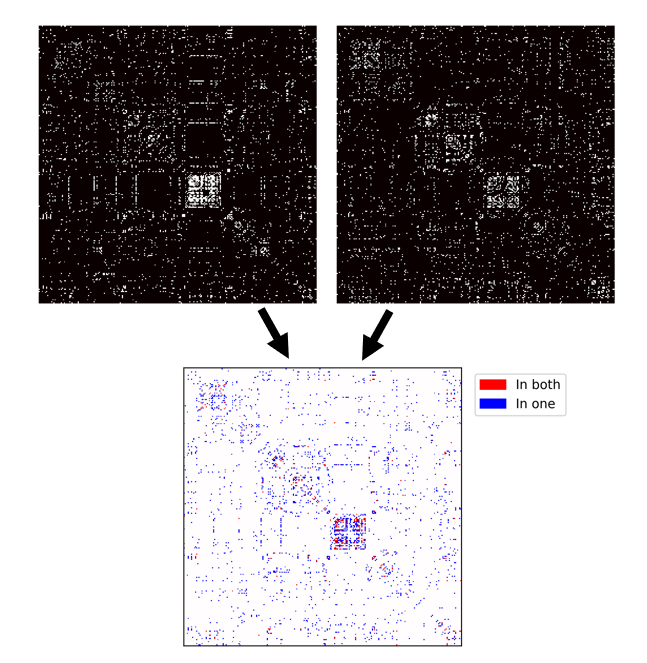
\includegraphics[height=3in]{ch4-network-intersection-methods}
    \caption[Method for comparing connectivity arrays.]{The network similarity measure provides a way of comparing connectivity arrays without reference to a pre-defined network parcellations.}
	\label{fig:ch4-network-intersection-methods}
\end{figure}

We first compared the mean similarities of network arrays across individuals within the two linguistic conditions: listening to listening and reading to reading. We summarized the distributions of these similarites, with the expectation that there would be the most variability within the reading condition, since listening is more ``natural''. Next, we tested whether the similarity between an individual's reading and listening network arrays was related to reading skill. Finally, we RSN-level patterns of similarity and difference between reading and listening, to identify both a common ``backbone'' and a flexible ``periphery''. 

Next, we broadened the scope of analysis to include comparisons between all task conditions: rest, attention, and passage (across both conditions). For each subject, we created a similarity matrix describing the shared connections between each of these conditions. Then, we extracted the mean and standard devation of the shared connections. The question we were interested in was whether, within-subject, individuals who had fewer changes in state were also better cognitive performers. We then sought to determine whether changes within a single RSN (e.g. the fronto-parietal network) were the key drivers of this. 

\section{Results}

\subsection{Behavioral results}

Attention and comprehension measures were not related to modality of stimulus presentation (see Fig. \ref{fig:ch4-task-performance}). There was a trend towards difference in median FDRMS between scan modalities (paired t-test, $t = 1.94$, $p = 0.059$), so we also replicated analyses with a stricter motion threshold (no more than 10 percent outliers in a scan run). The main results from analysis of this 35 subject (116 scan runs) cohort were broadly consistent.

\begin{figure}[t]
	\centering
	\includegraphics[height=3in]{ch4-task-performance}
    \caption[Behavioral metrics of passage performance were unrelated to modality.]{Both the in-scanner comprehension question and out-of-scanner recall questionnaire were unrelated to the modality of presentation.}
	\label{fig:ch4-task-performance}
\end{figure}

\subsection{Activation results}

As expected, reading and listening shared a common core of language-related activations. These included the bilateral middle temporal and inferior frontal gyri, as well as the  anterior temporal poles. The differences related to modality fell into three categories: sensory processing areas, including the insula, superior temporal gyrus, and secondary visual processing areas; and hetero-modal association areas, most notably the inferior frontal gyrus and angular gyrus; and somato-motor regions, including the premotor cortex and lateral geniculate nucleus of the thalamus (Fig. \ref{fig:ch4-modality-comparison-rest}). Areas showing greater activation in listening were focused on primary auditory cortex and the dorsal attention network.

\begin{figure}[t]
	\centering
	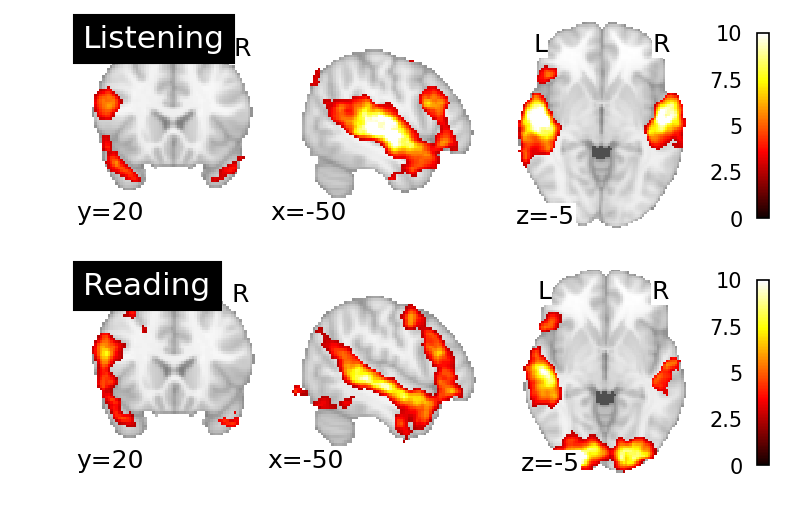
\includegraphics[height=3in]{ch4-modality-comparison-rest}
    \caption[Large overlap between listening and reading activation.]{Both the in-scanner comprehension question and out-of-scanner recall questionnaire were unrelated to the modality of presentation.}
	\label{fig:ch4-modality-comparison-rest}
\end{figure}

This result is more easly visualized when viewing it in terms of the 264 nodes of the connectome (Fig. \ref{ch4-modality-comparison-rest-connectome}). There was a very high correlation coefficient ($r < 0.001$), reflecting the high degree of shared activity patterns between listening and reading. In general, areas that are active during listening are also active during reading, with the main differences falling into the sensory networks. 

\begin{figure}[t]
	\centering
	\includegraphics[height=3in]{ch4-modality-comparison-rest-connectome}
    \caption[Large overlap between listening and reading activation in the connectome space.]{When projected into the node space, there was very strong correlation between activity in one and the other.}
	\label{fig:ch4-modality-comparison-rest-connectome}
\end{figure}

\subsection{Network results}

In terms of graph theory measures, we found a significant decrease in modularity and a significant increase in path length in reading compared to listening. This reflects that greater demands of reading, especially visually. This is displayed in Figure \ref{fig:ch4-modality-graph-theory}.

\begin{figure}[t]
	\centering
	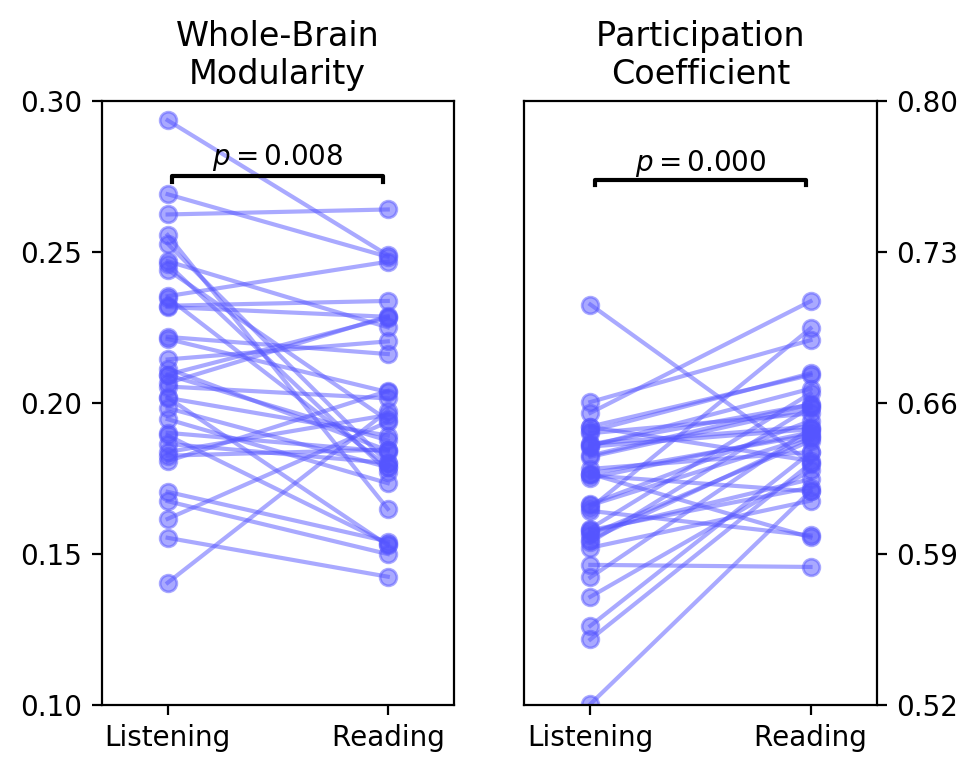
\includegraphics[height=3in]{ch4-modality-graph-theory}
    \caption[Large overlap between listening and reading activation in the connectome space.]{When projected into the node space, there was very strong correlation between activity in one and the other.}
	\label{fig:ch4-modality-graph-theory}
\end{figure}

For the modality contrast, one of the main takeaways is that there is greater access between auditory and other areas during reading. this runs counter to our hypothesis that there would be less access to these areas. Visual areas, on the other hand, show less internal connectivity, reflecting the de-clustering of these areas during reading. This is presented in Figure \ref{fig:ch4-modality-reorganization}.

\begin{figure}[t]
	\centering
	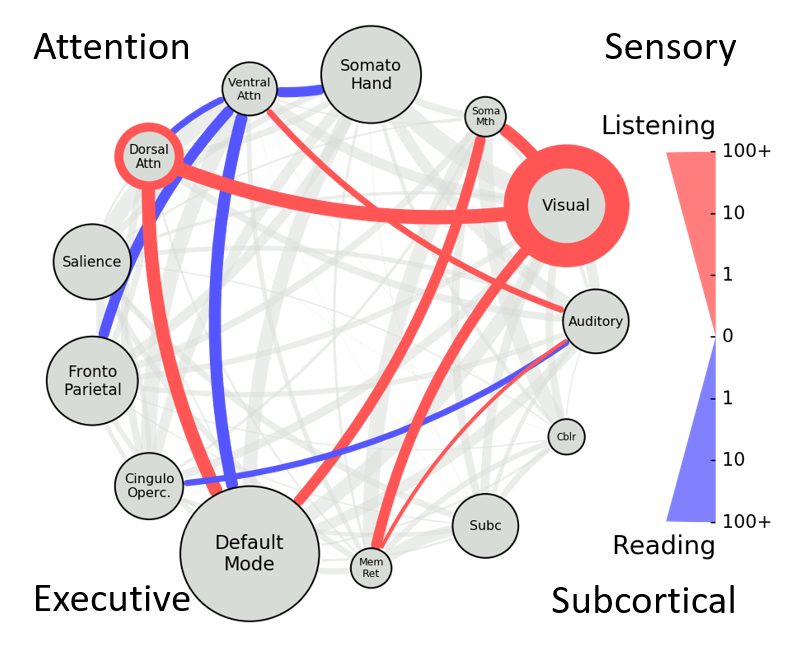
\includegraphics[height=3in]{ch4-modality-reorganization}
    \caption[Large overlap between listening and reading activation in the connectome space.]{When projected into the node space, there was very strong correlation between activity in one and the other.}
	\label{fig:ch4-modality-reorganization}
\end{figure}

\subsection{Network similarity results}



\begin{figure}[t]
	\centering
	\includegraphics[height=3in]{ch4-similarity-matrix-all}
    \caption[Auditory network organization is more similar for all subjects than it is for reading.]{}
	\label{fig:ch4-modality-network-similarity}
\end{figure}


\begin{figure}[t]
	\centering
	\includegraphics[height=3in]{ch4-similarity-matrix-reading}
    \caption[Network similarity between listening and reading predicts word efficiency.]{When projected into the node space, there was very strong correlation between activity in one and the other.}
	\label{fig:ch4-modality-network-similarity}
\end{figure}


\begin{figure}[t]
	\centering
	\includegraphics[height=3in]{ch4-similarity-matrix-reading}
    \caption[Diversity of between-network connections predominates on .... ]{Subjects that have more modular architectures are able to do it through greater hub... }
	\label{fig:ch4-modality-network-similarity}
\end{figure}

% Look at nodes that show increased participation coefficient across each different task. 



\section{Discussion}

The current study sought to determine whether aspects of the brain's network architecture are related to reading. The results suggest that an efficient network organization, i.e. one in which brain areas form clusters connected by hub regions, is important for skilled reading, and that dyslexia can be characterized by abnormal functioning of hub regions that map information between multiple systems. To our knowledge, this is the first time the relationship between modularity and hubness to reading skill has been described, adding to a foundation of work built on other connectivity methods.

A connectomics approach to reading illuminates -- not displaces -- previous neuroimaging research, much of which focused on localizing specific cognitive processes. One insight is that much of the ``reading network'' falls in domain-general RSNs such as the attention and executive networks (see Fig. 1). While these areas perform a specific function in reading, they are also often involved in other processes. For example, the dorsal attention network (DAN) encompasses the visual word form area, an area that has been the subject of much interest and debate in reading and dyslexia research \citep{McCandliss2003}. It is probable that this area is so important in reading not only because it is connected to language areas \citep{Bouhali2014}, but also because it is tightly tied to other areas that control goal-directed attention \citep{Vogel2014}. Koyama et al. (2013) found that children with a historical diagnosis of dyslexia had persistent de-coupling of the DAN compared to typical readers regardless of remediation status \citep{Koyama2013}. Vogel et al. (2012) found that reading ability in typical children and adults (including decoding and passage comprehension ability) predicted increased correlations between the visual word form area and the DAN \citep{Vogel2012a}. The nesting of this orthographic-processing area within the DAN is thus important to its role in reading.

An efficient small-world organization in the resting brain requires a modular network architecture, which was tied here to better performance in reading. This relationship was particularly high in the visual, default mode, cingulo-opercular networks. It is not yet possible to say whether modularity within these specific RSNs correlates most highly with reading because of their functional roles in reading processes or whether they simply capture global trends better than other networks. There is some reason to suspect specificity, however. In studies of remediation-induced changes to connectivity, increased connectivity within the visual network \citep{Koyama2013} and cingulo-opercular network \citep{HorowitzKraus2015} have predicted reading improvement in dyslexic children. The default mode network, on the other hand, supports a wide range of cognitive processes important for comprehension, including theory of mind, narrative processing, and autobiographical recall \citep{Buckner2008, AbdulSabur2014}, and its cohesiveness during resting-state has been used to investigate other disorders \citep{Uddin2008}. Future work will need to examine not just the internal connectivity, but the relationships between these networks during reading and at rest. The default mode network, for example, is typically anti-correlated with "task-positive" networks such as the fronto-parietal network. A high degree of anti-correlation has been reported to be important for performance on a variety of cognitive processes \citep{Fox2005, Keller2015}, but recent work suggests that high modularity and connectivity of the default mode during higher-level cognition is fundamental to processes relying on self-referential and memory retrieval processes, such as those found in language \citep{Vatansever2015}. The dynamics behind these interactions will be important for further establishing a framwork for investigating the roles of specific networks during reading. 

The additional findings that hubs areas are key in dyslexia are not surprising: dyslexia has often been thought to be a disorder of combining information across different functional systems, and in the context of connectomics, hub areas play a privileged role in mediating information flow between RSN’s. For example, the posterior temporal sulcus connects visual and auditory networks by binding letters to sounds \citep{Blau2010, VanAtteveldt2009} and the inferior frontal gyrus has many different subdivisions supporting language parsing and manipulation \citep{Hagoort2005}. However, casting dyslexia dysfunction into a connectomics perspective opens up new hypotheses and research avenues. For example, the brain areas of interest and neuroimaging metrics can be unified across other developmental disorders, including ADHD, specific language impairment and autism \citep{Stam2014}. Another benefit is that it opens up many more avenues for investigating dyslexia using functional and diffusion MRI, which can be performed in younger children and without administering a cognitive task. 